\documentclass{article}

\usepackage{stmaryrd}
\usepackage{amsmath}
\usepackage{amssymb}
\usepackage{amsthm}
\usepackage{relsize} 
\usepackage{bm} 
\usepackage{IEEEtrantools}
\usepackage{graphicx}
\usepackage[font={small,it}, width=\textwidth]{caption}
\usepackage{subcaption}
\usepackage{hyperref}
\usepackage{cases}
\usepackage{xfrac}
\usepackage{comment}
\usepackage{framed}
\usepackage[ ddmmyyyy ]{datetime} 
\usepackage{fancyhdr}
\usepackage{enumitem}
\usepackage{cite}
\usepackage{float}
\usepackage{multirow}

\newcommand{\source}[1]{\caption*{\hfill Source: {#1}} }

\usepackage{mathtools}
\DeclareMathOperator{\sign}{sign}
\DeclareMathOperator{\sat}{sat}

\oddsidemargin = 20pt
\textwidth = 420pt

\hypersetup{
     colorlinks   = true,
     linkcolor    = blue
}

\title{Dual Motor Control}
\author{Marcus Greiff}

\begin{document}
\maketitle

\section{Introduction}

\subsection{Cart model}
The most basic cart model consists of simply setting up the equations of motion for the cart with the motor torques as input signals,
\begin{equation}\label{eq:motion}
M\ddot{x} = \frac{u_1+u_2}{d} - F_f(\dot{x}).
\end{equation}
Here, the control signals $u_1$ and $u_2$ are the torques generated by the two motors, $d$ is the cart wheel radius and $M$ is the cart mass. In this simple linear model, the friction force, $F_f(\dot{x}) = b\dot{x}$, is simply proportional to the cart speed with some constant $b$. By introducing the state variables $\mathbf{x} = [x, \dot{x}]^T$ and letting the control signal $\mathbf{u} = [u_1, u_2]^T$, the system can be written as
\begin{equation}\label{eq:linModelCart}
\dot{\mathbf{x}} = \mathbf{A}_c\mathbf{x} + \mathbf{B}_c\mathbf{u} =
\begin{bmatrix}
0 & 1\\
0 & b/M
\end{bmatrix}\mathbf{x}  + 
\frac{1}{Md}
\begin{bmatrix}
0 & 0\\
1 & 1
\end{bmatrix}\mathbf{u},
\end{equation}
This state space representation was used to derive certain controllers, but does not take the many non-linearities of the system into account, most notably the backlash, motor torque saturation and non-linear friction. In the original model implementation (see Figure~\ref{fig:SimModel}), the linear dynamics were implemented separate to the non-linearities in order to investigate their effect separately. However, in the open source project, a simpler linear cart was implemented to show the effect of the non-linear torque splitting and how the cascade control loop is constructed (see \texttt{DMC.slx}).

\begin{figure}[htbp]
\centering
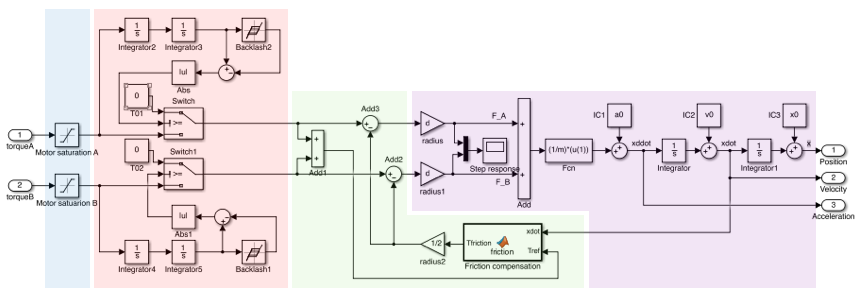
\includegraphics[width=0.9\textwidth]{figures/CartSimulink.png}
\rule{35em}{0.5pt}
\caption{The Simulink cart model with motor torque saturation (blue), the backlash model (red), the non-linear friction model (green) and the linear cart dynamics (purple).}
\label{fig:SimModel}
\end{figure}

\subsection{Backlash compensation}
As this work aspires to be reused in parallel kinematics projects, the complete dynamics of the final robot will be very different from that of a simple cart. In order for the backlash compensation to be reusable, it should therefore be largely independent of system dynamics. Consequently, approaches such as those using state-dependent algebraic Ricatti equation (SDARE) method cannot be used~\cite{friedland1997feedback}. Instead, a simple non-linear filter is proposed to (i) operate the motors synchronously at large reference offsets to improve the system response, and (ii) to operate the two motors in the opposing directions when the reference offset is small to completely get rid of backlash and improving accuracy in stationarity. This method of compensation is more economical in terms of power consumption than the method described in a Cairen's thesis on DMC control ~\cite{Patrik:2013}, where the motors were working in opposing directions at all times. 

The non-linear filter exploits the fact that the effective force applied to the cart, $u$, is proportional to the sum of the motor torques, $T_a$ and $T_b$. As long as there exists good torque control of the motors and the controllers are tuned equally, we may perturb the motor torques slightly by some constant, $\epsilon_{bw}$, and still achieve the same effective force
\begin{equation}\label{eq:splitEq}
\frac{u_1 + u_2}{d}  = \frac{\sat(T_a) + \sat(T_b)}{d} = \frac{\sat(T_a +  \epsilon_{bw}) + \sat(T_b - \epsilon_{bw})}{d}.
\end{equation}
This statement holds only when absolute value of the perturbed torque reference is within the bounds of saturation, but proves no issue for our application, as $\epsilon_{bw} << \max_t(|T_a|,|T_b|)$ and the absolute saturation limit can be lowered by $\epsilon_{bw}$ to guarantee that~\eqref{eq:splitEq} holds. As we only include feed forward terms of acceleration, velocity and position, we denote the $i^{th}$ derivative of the control error by $e^{(i)}(t) = x^{(i)}(t)  - x^{(i)}_{ref}(t)$ and let $\tilde{e}(t) = \max_i(|e^{(i)}(t)|)$ with $r = 2$. Using equation~\eqref{eq:splitEq}, we then demand that $T_a = T_b$ when the control error is above some threshold $\tilde{e}(t) > \epsilon_{th}$, and that reference torques are only split continuously for smaller control errors, such that $\tilde{e}(t) \equiv 0\Rightarrow T_a = -T_b \Rightarrow u_1 + u_2 = \epsilon_{bw}-\epsilon_{bw} = 0$. With this approach, both conditions (i) and (ii) will be satisfied, eliminating backlash completely when all control error derivatives are small. In summary the filter function, $f(u,e)$, has to be chosen so that $f(u,0) = \epsilon_{th}$ and $f(u,\epsilon_{bw}) = 0$, and general filter can then be written
\begin{equation}
h(u,e) = 
\begin{cases}
\tilde{e}(t) = \max\limits_{i = 0,...,r}(|e^{(i)}(t)|) \quad r\in\mathbb{N}_0\\
\frac{1}{2}\{u, u\} \qquad\qquad\qquad\quad\;\; \text{if}\; |\tilde{e}(t)| > \epsilon_{th}\\
\frac{1}{2}\{u \pm f(u,\tilde{e})\} \qquad\quad\quad\;\;\text{if}\; |\tilde{e}(t)| \leq \epsilon_{th}\\
\end{cases}
\;\;\text{where}\;\;\epsilon_{th},\epsilon_{bw}\in \mathbb{R}_+,\;\; \epsilon_{th}\leq\epsilon_{bw}
\end{equation}
An initial linear filter function,
\begin{equation}
f_1(u,\tilde{e}) = \epsilon_{bw} \cdot (\epsilon_{th}  - u \cdot \sign(\tilde{e})) \in C^1,
\end{equation}
was implemented in Simulink and simulated with good results, but behaved strangely with certain control schemes (notably second order sliding mode control) due to it not having a second derivative. To remedy this, the conditions $f^{\prime}(0) = f^{\prime}(\epsilon_{bw}) = 0$ were enforced, and a trigonometric function was used instead of a linear one (see Figure~\ref{fig:filter}), making the filter smooth and continuous in the $n^{th}$ derivative,
\begin{equation}
f_2(u,\tilde{e}) = \frac{\epsilon_{bw}}{2}\Big(1+\cos\Big(\frac{\pi \tilde{e}}{\epsilon_{th}}\Big)\Big) \in C^N.
\end{equation}
Note that this ``$C^N$-filter" can be implemented such that the control error is with reference to position, velocity, acceleration or a combination of the three.

\begin{figure}[htbp]
\centering
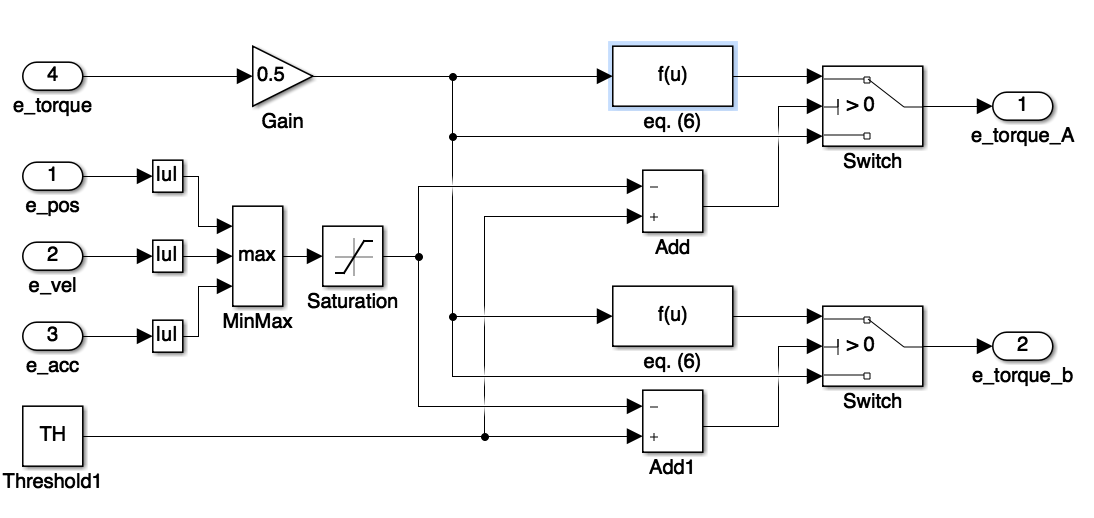
\includegraphics[width=0.7\textwidth]{figures/CN_filter.png}
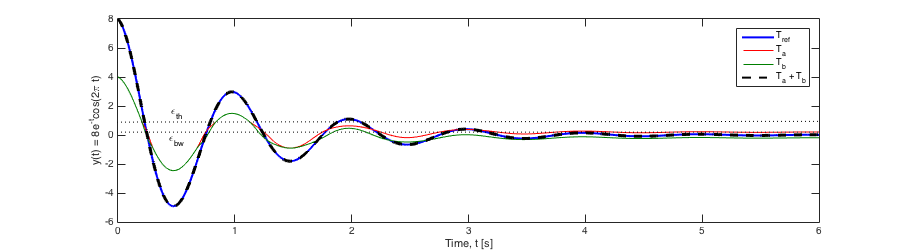
\includegraphics[width=0.9\textwidth]{figures/CNFILT.png}
\rule{35em}{0.5pt}
\caption{\textbf{Top:} The simulink implementation of the  $C^N$-filter with $r=2$. \textbf{Bottom:} The $C^N$-filter with $r=0$ applied to the input $u(t) = 8e^{-t}cos(2\pi t)$ (blue), with the outputs $T_a$ (red) and $T_b$ (green), and the sum of the outputs (black). The splitting is done when the positional error is small, and approaches a stationary split $T_a=-T_b$ when $e\approx 0$.}
\label{fig:filter}
\end{figure}

\subsection{Trajectory planning}
The trajectory planning has two separate functions. The first is to simply to take reference function of position, velocity or acceleration, and then generate the signals required in the feed-forward loop. For example, if a sinusoidal velocity reference is to be followed, the trajectory planner should evaluate and output velocities in time, as well as it's derivative (acceleration) and primitive (position). The second mode of operation is to detect sudden reference changes in position ( steps), and then approximate a fourth degree reference polynomial which moves the cart to the required position in optimal time given constraints on velocity, $\hat{v}$, acceleration, $\hat{a}$, and jerk, $\hat{j}$, and jerk derivative, $\hat{d}$. The first problem is trivial, but the second is more difficult can be formulated mathematically as
\begin{equation}\label{eq:optProb}
\text{Minimize}(t_f)\;\;\text{ subject to}\;\;\\
\begin{cases}
x(t_0) = r_0, x(t_f) = r_f\\
\dot{x}(t_0) = \ddot{x}(t_0) = x^{(3)}(t_0) = x^{(4)}(t_0)=0\quad (*)\\
\dot{x}(t_f) = \ddot{x}(t_f) = x^{(3)}(t_f) = x^{(4)}(t_f) = 0 \\
|x^{(4)}(t)|<\hat{d},|x^{(3)}(t)| < \hat{j}, |\ddot{x}(t)|<\hat{a}, |\dot{x}(t)| <\hat{v} \quad(**)\\
\end{cases}
\end{equation}
by defining the time of a change in reference as $t_0 = 0$, and the time at which the new reference position is reached as $t_f > t_0$. Here, $r_0$ is the positional reference before $t_0$ and $r_f$ is the desired position. We also require the jerk and all lower derivatives to be continuous at all times. In future iterations, it is worth considering setting the derivatives at $t_0$ as free variables $(*)$, to properly allow the computation of new reference steps while the cart is moving. Here we make the assumption of $(*)$ and use the symmetry of the problem, to which the general solution is a set of polynomial splines of order $p\leq4$,
\begin{equation}\label{eq:gensol}
\begin{cases}
x^{(4)}(t) = d_i\\
x^{(3)}(t) =  d_it+j_i\\
\ddot{x}(t) = \dfrac{{d_i}}{2}t^2 + {j_i}t + a_i\\
\dot{x}(t) = \dfrac{{d_i}}{6}t^3 + \dfrac{{j_i}}{2}t^2 + {a_i}t + v_i\\
x(t) = \dfrac{{d_i}}{24}t^4 + \dfrac{{j_i}}{6}t^3 + \dfrac{{a_i}}{2}t^2 + {v_i}t + x_i.
\end{cases}
\end{equation}
These splines exist on a time interval $[t_i,t_{i+1}]$, and are defined as sets $S_i = \{d_i, j_i, a_i, v_i, x_i,t_i, t_{i+1}\}$, and the idea is to start simple and then introduce the constraints $(**)$ one by one. Due to the boundary conditions on velocity, the acceleration has to be zero at $t=t_f/2$, which implies that the jerk has to be zero at  $t = t_f/4,2t_f/4,3t_f/4$. It is then clear that the jerk derivative must be alternating between $x^{(4)}(t)=\pm\hat{d}$ on eight equidistant time intervals, $t_d$. 
The jerk derivative in each spline $S_i$ is then given by the corresponding element in the vector
\begin{equation}\label{eq:djerksol}
\mathbf{d} = \sign(r_f - r_0)\cdot\hat{d}\cdot[1,-1,-1,1,1,-1,1]\\
\end{equation}
where 
\begin{equation}\label{eq:djerkref}
t_d=\sqrt[4]{\dfrac{|r_f - r_0|}{8\hat{d}}},
\end{equation}
is determined from~\eqref{eq:gensol} and the remaining constants are chosen to preserve continuity. When adding the remaining constraints $(**)$, we need to introduce periods of constant jerk of length $t_j$, constant acceleration of length $t_a$ and constant velocity of length $t_v$, such that the constraints are preserved. The general solution is then 
\begin{equation}
\begin{cases}\label{eq:fullsol}
\mathbf{d} = \sign(r_f - r_0)\cdot\hat{d}\cdot[1,0,-1,0,-1,0,1,0,1,0,-1,0,1]\\
\mathbf{t} =[t_d,t_j,t_a,t_j,t_d,t_v,t_d,t_j,t_a,t_j,t_d,]
\end{cases}
\end{equation}
where the jerk derivative and time interval length in each spline $S_i$ is given by the corresponding element in $\mathbf{d}$ and $\mathbf{t}$ respectively. The time interval lengths and splines are then determined in five steps.

\subsubsection*{Step 1}
We start by finding $t_d$, as the maximum time that the jerk derivative can be kept zero separate without violating $(**)$, which is given by
\begin{equation}\label{eq:td}
t_{d} = \min\begin{Bmatrix}\sqrt[4]{\dfrac{|r_f - r_0|}{8\hat{d}}}, \sqrt[3]{\dfrac{\hat{v}}{2\hat{d}}}, \sqrt{\dfrac{\hat{a}}{\hat{d}}},\dfrac{\hat{j}}{\hat{d}}\end{Bmatrix}
\end{equation}
as the initial conditions on the derivative terms are $\mathbf{x}(t_0) = \mathbf{0}$. Now, if $t_d$ depends on the first term (i.e. the index of the minimum value in ~\eqref{eq:td} is 1), we violate a constraint on jerk derivative and nothing else, and the solution takes the form of ~\eqref{eq:djerksol} described above with $t_j=t_a=t_v=0$. If the jerk is first violated (index 2), we need to introduce periods of constant jerk, shown in \textbf{Step 2}. If the acceleration is first violated (index 3), $t_j = 0$, and we proceed with \textbf{Step 3}. Finally, if the constraint on velocity is first violated (index 4), $t_j=t_a=0$, and we compute a period of constant velocity in \textbf{Step 4}.

\subsubsection*{Step 2}
According to~\eqref{eq:gensol} and~\eqref{eq:fullsol}, the maximum $t_j$ at which the constraint $|x^{(3)}(t)| < \hat{j}$ is still satisfied, is given by the real and positive solution to
\begin{equation}\label{eq:tjj}
t_j^3 + 5t_dt_j^2 + 8t_d^2t_j + 4t_d^3-\dfrac{|r_f - r_0|}{2\hat{d}t_d} = 0.
\end{equation}
This choice of $t_j$ ensures that we arrive at the correct terminal point, $x(t_f) = r_f$. However, we must also check if the constraint on acceleration and velocity is violated. By examining~\eqref{eq:gensol} and~\eqref{eq:fullsol}, these constraints are violated exactly when
\begin{equation}\label{eq:tja}
\sup\limits_{t_0\leq t\leq t_f}|\ddot{x}(t)| = \hat{a} \Rightarrow t_j = \dfrac{\hat{a}- \hat{d}t_d^2}{\hat{j}}.
\end{equation}
and for the velocity
\begin{equation}\label{eq:tjv}
\sup\limits_{t_0\leq t\leq t_f}|\dot{x}(t)| = \hat{v} \Rightarrow
\hat{j}(t_d + t_j)t_a + \hat{d}(t_d^3 + t_d^2t_j)+ \hat{j}(2t_jt_d + t_j^2+t_d^2)-\hat{v} =0
\end{equation}
The smallest real solution $tj>0$ to ~\eqref{eq:tjj}~\eqref{eq:tja}~\eqref{eq:tjv} is chosen so that the solution complies with all constraints.
If this $t_j$ is given by the constraint on jerk ~\eqref{eq:tjj}, we arrive at our terminal point keeping all constraints in $(**)$ and we are done.
If $t_j$ is given by the constraint on acceleration ~\eqref{eq:tja}, we proceed with \textbf{step 3}, and if the constraint on velocity~\eqref{eq:tjv} is violated first, $t_a = 0$ and we move straight to \textbf{Step 4}.

\subsubsection*{Step 3}
A period of constant acceleration, $t_a$, is computed such that the terminal point $x(t_f) = r_f$. This time is given by the real an positive solution to
\begin{equation}
(t_d^2+t_dt_j)t_a^2+
(6t_d^3+9t_d^2t_j+3t_dt_j^2)t_a+
8t_d^4+16t_d^3t_j+10t_d^2t_j^2+2t_dt_j^3-\dfrac{|r_f - r_0|}{\hat{d}} = 0
\end{equation}
as derived from equation~\eqref{eq:gensol} and~\eqref{eq:fullsol}. However, we might then violate the velocity constraint, and must therefore compute the $t_a$ at which the maximum velocity is reached. This is done by solving~\eqref{eq:tjv} for $t_a$. Just as in \textbf{Step 2}, if the constraint on velocity is not breached, the algorithm arrives at the terminal point and we are done. If the velocity constraint is violated (i.e. $t_f$ is given by~\eqref{eq:tjv}) we proceed with \textbf{Step 4}.

\subsubsection*{Step 4}
Here, a period of constant velocity, $t_v$, is introduced. No $t_v>0$ can violate any of the constraints in $(**)$ since the speed is constant during $t_f$, and the period time is simply computed so that  $x(t_f) = r_f$. This can either be done similarly to $t_j$ and $t_a$, by finding $t_v$ analytically from~\eqref{eq:gensol} and~\eqref{eq:fullsol}. In the implementation, this is done automatically in \textbf{Step 5} by checking the end point position, $x_p$, and velocity, $v_p$, of the 7th spline and computing $t_v = x_p/v_p$.

\subsubsection*{Step 5}
In this final step, the splines are created based on $~\eqref{eq:fullsol}$ to preserve continuity in all derivatives between the splines. In doing so, a complete trajectory can be generated in the cycle where the positional reference step is taken (see the function block \texttt{computeTrajectory}), and then evaluated at a given point in time (see the function block \texttt{evaluateTrajectory}). This approach was taken to decrease the computational effort and allow a higher cycle frequency.

\begin{figure}
\centering
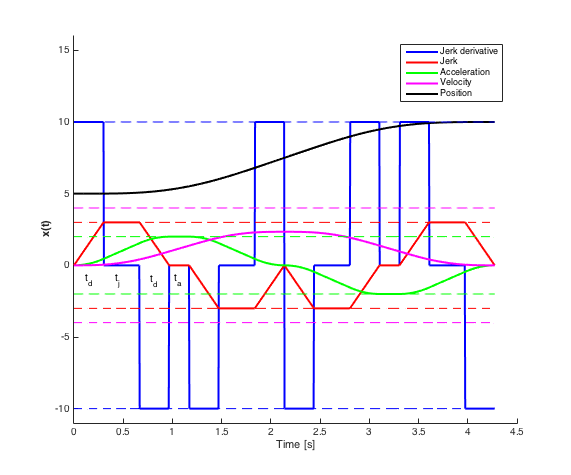
\includegraphics[height = 6cm, width = 0.7\linewidth]{figures/Splines.png}
\rule{35em}{0.5pt}
\caption{The fourth order trajectory generated for a positional reference step from $r_0 = 5$ to $r_f=10$ [cm] at the time $t_0 = 0$, given the bounds $[\hat{d},\hat{j},\hat{a},\hat{v}]= [10,3,2,4]$ (dashed). The optimal time given the harsh constraints is $t_f\approx 4.3$.}
\label{fig:posref}
\end{figure}

\clearpage\subsection{Cart control}
Since previous work done in backlash compensation using DMC and positional PID control resulted in a very low repeatable positional accuracy, this method was used as a starting point in the controller design~\cite{Patrik:2013}. However, this gave bad results when implemented in TwinCAT, and was not investigated further due to a lack of time. Instead, two  approaches commonly used in the industry for rigid robotics, the feed-forward PID-control and the cascade control, were implemented in Simulink to make use of the information generated by the trajectory planner (see Figure ~\ref{fig:controlSimulink})~\cite{PID2015feedforward}.

\begin{figure}
\centering
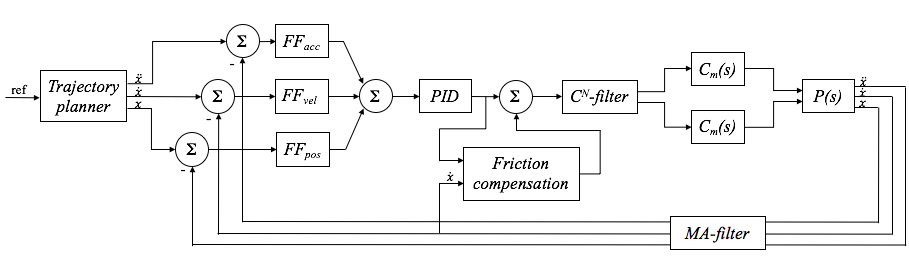
\includegraphics[width = 0.8\linewidth]{figures/PIDfeed-forward.png}
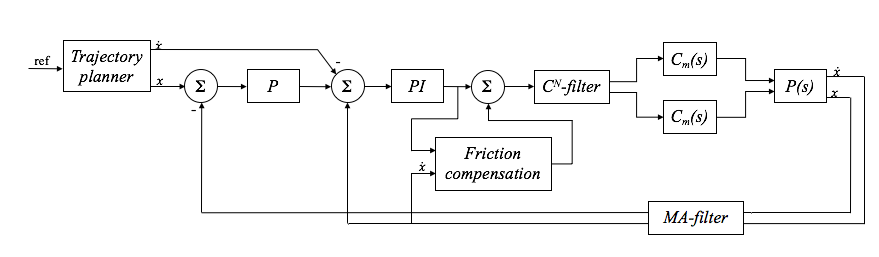
\includegraphics[width = 0.8\linewidth]{figures/CascadeControl.png}
\caption{The feed-forward PID control  (top) and the cascade control (bottom) as implemented in Simulink.}
\label{fig:controlSimulink}
\end{figure}

In the physical process, the two motors of the cart are controlled by a pair of EPOS3 70/10 drivers developed by Maxon. These drivers can be configured to have the motor follow various reference signals, such as position, velocity and torque. Given the structure of the $C^N$-filter, the PID-controlled current loop over the motors was auto-tuned to follow a reference torque.

A model of the asynchronous squirrel cage motors was created in Simulink using the ``asynchronous macine'' based on the work of Li et al. (see \texttt{motor\_model.slx}, Gitlab)~\cite{li2013modeling}. Due to the poor data sheet of the motors, there were too many unknown parameters to make good use the motor model when simulating the system. Consequently, for the purpose of crude simulations of control in Matlab, the driver control loop was omitted and a 1:1 relation of reference torque and actual motor torque was assumed.

In the feed-forward scheme, the control errors in position, velocity and acceleration are amplified by feed forward gains and summed in to a single error signal. This error is fed to the PID control, which in turn generates a control signal corresponding to an effective total motor torque. After the friction compensation, the signal control is split by the $C^N$-filter and fed to the motor drivers as reference torques.

In the cascade control, a P-PI loop is used to to compensate errors in position and velocity successively. Simulations showed that good control could be achieved both when using the P-PI loop (see FIgure~\ref{fig:controlSimulink}), that both speed and accuracy could be increased by introducing a second PI-term on acceleration. However, this P-PI-PI control could not be realized in TwinCAT due to noisy signals and highly inaccurate acceleration measurements. 

The tuning of the P-PI loop was relatively simple in Matlab but proved very difficult in the real process. In order to both have good transient behavior and make the cart follow it's optimal trajectory, gain scheduling was used to increase the P-parts on position and velocity while moving the cart, and scaling down both P-gains by a factor of 100 when approaching the reference position (see Figure ~\ref{fig:CascadeControl}). In addition, error in velocity was completely disregarded when below a certain tolerance if also the positional error of an order of a few mm. In doing so, integral action work exclusively on positional control.

\begin{figure}
\centering
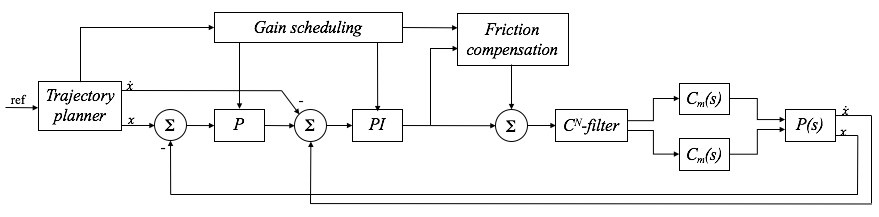
\includegraphics[width = 0.8\linewidth]{figures/CascadeTwincat.png}
\caption{The cascade control as implemented in Simulink (top) and TwinCat (bottom).}
\label{fig:CascadeControl}
\end{figure}

\subsection{Anti-Windup}
When running the physical process with the P-PI cascade control and the trajectory planning set to only constrain jerk derivative, small positional oscillations were present as the cart approached the terminal trajectory position, $r_f$ (see the torque control signals in \textbf{Section 5}, Figure~\ref{fig:torquesplit}). In order for the cart to reach a stable position in a short amount of time, the influence of the oscillations had to be minimized. When investigating the problem, it seemed largely dependent on the I-gain. This was confirmed in the Simulink model, where the behavior was replicated when using cascade control with high I-gains along with third order trajectory planning (see Figure~\ref{fig:AntiWindupResults}). Here the oscillations are most clearly visible in the plot of acceleration and velocity, and significant enough to cause large position errors when compared to the desired repeatable accuracy on the micrometer scale.
\begin{figure}
\centering
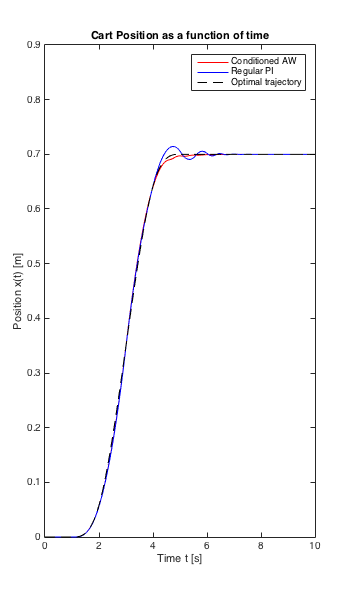
\includegraphics[width = 0.3\linewidth,height=6cm]{figures/PositionAW.png}%
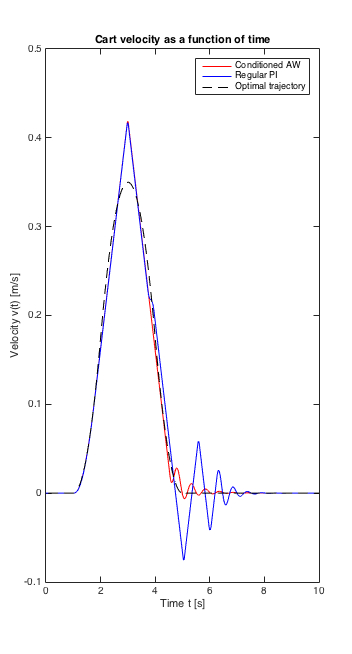
\includegraphics[width = 0.3\linewidth,height=6cm]{figures/VelocityAW.png}%
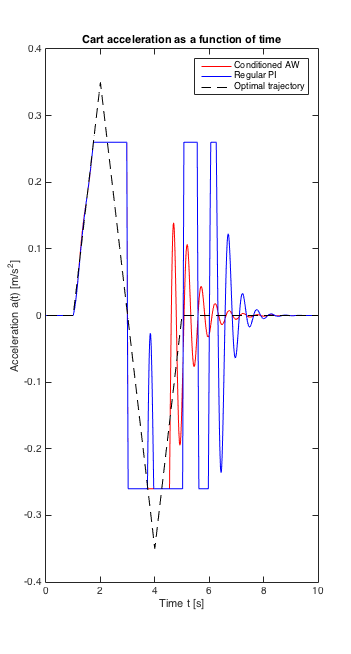
\includegraphics[width = 0.3\linewidth,height=6cm]{figures/AccelerationAW.png}
\caption{Cart position (left), velocity (center) and acceleration (right) when running the cart model along a third-order trajectory (black, dashed) with conditioned AW P-PI cascade control, and regular P-PI cascade control.}
\label{fig:AntiWindupResults}
\end{figure}

A good way of mitigating the oscillatory behavior induced by $I$-gain is to use one of many anti-windup schemes (AW). Four different approaches were investigated, based on the work on J. Espina et al.~\cite{espina2009speed}. In this survey of fast AW schemes, the authors concluded that for PI-control of permanent magnet synchronous machines, the conditioned AW had the lowest settling time and overshoot of the methods considered. This conditioned AW scheme simply detects when the control signal gets saturated, which in our case is when difference in reference torque before and after saturation is non-zero. In this state, the integrator holds it's most recent value. The conditioned AW scheme was implemented in Simulink using the memory block and a relational operator for checking when the control is saturated (see Figure ~\ref{fig:AntiWindupSimulink}). Note that the $D$-term was included with a filter-coefficient $N$ for the purpose of testing AW PID control, but that the $D$-gain was set to zero in the cascade control implementation. As expected, the oscillations are greatly suppressed and we reach stable desired position much faster than with conventional $PI$-regulators.

\begin{figure}
\centering
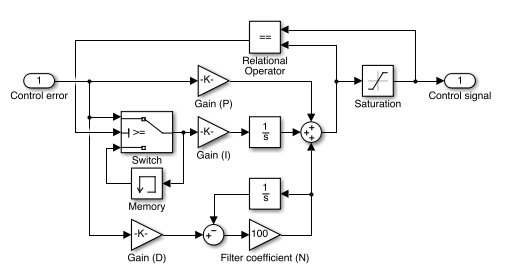
\includegraphics[width = 0.5\linewidth]{figures/AntiwindupSimulink.png}
\caption{The Simulink model of the continuous time conditioned AW-PID regulator.}
\label{fig:AntiWindupSimulink}
\end{figure}

The simulation was run with rough estimations of parameters such as the cart mass and motor rotor inertia, and was merely used to determine the effect of conditioned AW control, which yielded a significant improvement in control. Due to lack of time, this was never implemented in TwinCAT, but it is definitely worth investigating in future iterations of the TwinCAT software.

\newpage\bibliography{Bibliography}{}
\bibliographystyle{IEEEtran}
\end{document}